% Epistemic Honesty in Predictive Systems: An Impossibility Result
% Beamer Presentation for Systopia Research Group
% January 9, 2025

\documentclass[aspectratio=169,11pt]{beamer}

% Theme and colors
\usetheme{Madrid}
\usecolortheme{default}
\setbeamertemplate{navigation symbols}{}
\setbeamertemplate{footline}[frame number]

% Packages
\usepackage{graphicx}
\usepackage{booktabs}
\usepackage{amsmath,amssymb}
\usepackage{tikz}
\usetikzlibrary{arrows.meta,shapes,positioning,patterns}

% Custom colors
\definecolor{anthblue}{RGB}{60,90,150}
\definecolor{warnred}{RGB}{180,60,60}
\definecolor{truthgreen}{RGB}{60,140,80}

% Title formatting - light text on dark background for contrast
\setbeamercolor{title}{fg=anthblue}
\setbeamercolor{frametitle}{fg=white}

% For speaker notes (uncomment to show notes on second screen)
% \usepackage{pgfpages}
% \setbeameroption{show notes on second screen=right}

\title{Epistemic Honesty in Predictive Systems}
\subtitle{An Impossibility Result}
\author{Systopia Research Group Talk}
\date{January 9, 2025}

\begin{document}

%==============================================================================
% OPENING SEQUENCE (5 min)
%==============================================================================
\section{Opening}

% No slide for opening question - presenter asks directly
% "How many of you have read incorrect information from an LLM?"

\begin{frame}{The Disclaimer}
    \begin{center}
        
\includegraphics[width=0.85\textwidth]{claude-disclaimer.png}

        \vspace{0.5em}
        \textit{``Users should not rely on Claude as a singular source of truth.''}
    \end{center}

    \note{
        Read aloud: "Users should not rely on Claude as a singular source of truth."

        "To learn more about how Anthropic's technology works..."

        They're telling you to check their research on making models more reliable.
        They're also telling you not to trust the model.

        The disclaimer links to: "Claude is providing incorrect or misleading responses"
        support article. They know. They're warning you. They have no fix.
    }
\end{frame}

\begin{frame}{The Gap}
    \begin{columns}
        \begin{column}{0.45\textwidth}
            \centering
            \textbf{\large Marketing}

            \vspace{1em}
            \textcolor{truthgreen}{``Helpful, harmless, and honest''}
        \end{column}
        \begin{column}{0.1\textwidth}
            \centering
            \Huge ?
        \end{column}
        \begin{column}{0.45\textwidth}
            \centering
            \textbf{\large Disclaimer}

            \vspace{1em}
            \textcolor{warnred}{``Users should not rely on Claude\\as a singular source of truth''}
        \end{column}
    \end{columns}

    \vspace{2em}
    \pause
    \begin{center}
        \textit{Can both be true? Is this gap temporary---or structural?}
    \end{center}

    \note{
        "This is the only software product in history where the manufacturer explicitly
        warns you the output is likely defective, yet provides no diagnostic tool to
        check it. That's an engineering failure, not a policy choice."
    }
\end{frame}

\begin{frame}{What We're Claiming}
    \begin{enumerate}
        \item<1-> \textbf{Intuition:} Fundamental limit on verifying agent beliefs when observing only output
        \vspace{0.5em}
        \item<2-> \textbf{Theorem shape:} For any bounded judge observing lossy output, $\exists$ indistinguishable dishonest strategy
        \vspace{0.5em}
        \item<3-> \textbf{Why it matters:} RLHF produces confident outputs that \textit{appear} honest while leaving internal incoherence intact
    \end{enumerate}

    \vspace{1em}
    \pause[4]
    \begin{block}{Scope}
        Verification impossibility, not honesty impossibility.\\
        We can't \textit{verify} it through this interface---not that systems can't \textit{be} honest.
    \end{block}

    \note{
        Critical framing (say explicitly): "If you believe this impossibility is wrong,
        the way to refute it is to show WHICH ASSUMPTION FAILS or to exhibit an
        interface that preserves epistemic state."

        Pre-commit the room here.
    }
\end{frame}

%==============================================================================
% THE FAMILIAR PAIN (2 min)
%==============================================================================
\section{The Familiar Pain}

\begin{frame}{Debugging Without Causality}
    \begin{center}
        % TODO: Tangled distributed system diagram or Lamport diagram with "???"
        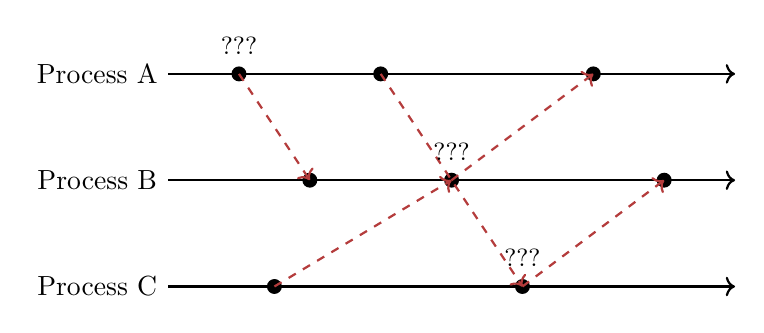
\begin{tikzpicture}[scale=0.9]
            % Processes
            \node (p1) at (0,3) {Process A};
            \node (p2) at (0,1.5) {Process B};
            \node (p3) at (0,0) {Process C};

            % Timeline arrows
            \draw[->, thick] (1,3) -- (9,3);
            \draw[->, thick] (1,1.5) -- (9,1.5);
            \draw[->, thick] (1,0) -- (9,0);

            % Events (dots)
            \fill (2,3) circle (3pt);
            \fill (4,3) circle (3pt);
            \fill (7,3) circle (3pt);
            \fill (3,1.5) circle (3pt);
            \fill (5,1.5) circle (3pt);
            \fill (8,1.5) circle (3pt);
            \fill (2.5,0) circle (3pt);
            \fill (6,0) circle (3pt);

            % Messages (tangled)
            \draw[->, dashed, thick, warnred] (2,3) -- (3,1.5);
            \draw[->, dashed, thick, warnred] (4,3) -- (6,0);
            \draw[->, dashed, thick, warnred] (5,1.5) -- (7,3);
            \draw[->, dashed, thick, warnred] (2.5,0) -- (5,1.5);
            \draw[->, dashed, thick, warnred] (6,0) -- (8,1.5);

            % Question marks for timestamps
            \node at (2,3.4) {\small ???};
            \node at (5,1.9) {\small ???};
            \node at (6,0.4) {\small ???};
        \end{tikzpicture}
    \end{center}

    \vspace{1em}
    \begin{center}
        \textit{You know this feeling. We built AI with the same problem.}
    \end{center}

    \note{
        "Logs without vector clocks. The causal structure existed at runtime.
        The system KNEW the ordering. But that knowledge wasn't preserved.
        The interface threw it away."
    }
\end{frame}

%==============================================================================
% THE EVIDENCE (10 min)
%==============================================================================
\section{Evidence}

\begin{frame}{What the Interface Shows}
    \begin{center}
        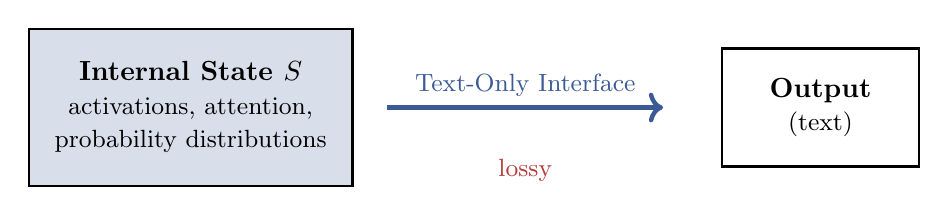
\begin{tikzpicture}
            % Internal state box
            \node[draw, thick, minimum width=4cm, minimum height=2cm, fill=anthblue!20] (internal) at (0,0) {
                \begin{tabular}{c}
                    \textbf{Internal State $S$}\\
                    \small activations, attention,\\
                    \small probability distributions
                \end{tabular}
            };

            % Narrow pipe
            \draw[->, ultra thick, anthblue] (2.5,0) -- node[above]{\small Text-Only Interface} (6,0);

            % Output
            \node[draw, thick, minimum width=2.5cm, minimum height=1.5cm] (output) at (8,0) {
                \begin{tabular}{c}
                    \textbf{Output}\\
                    \small (text)
                \end{tabular}
            };

            % Lossy annotation
            \node[warnred] at (4.25,-0.8) {\small lossy};
        \end{tikzpicture}
    \end{center}

    \vspace{1em}
    Everything inside the box gets compressed through this pipe.\\
    What doesn't fit gets thrown away.

    \note{
        "This is the observation model. Everything that follows depends on this constraint."
    }
\end{frame}

\begin{frame}{The Decoder Ring: A Taxonomy of Epistemic Failure}
    \begin{center}
    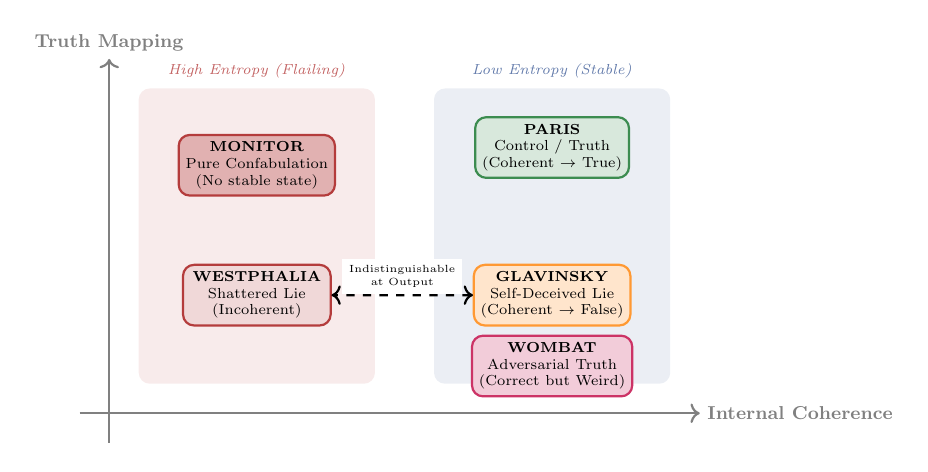
\begin{tikzpicture}[scale=0.75, transform shape]
        % Axes
        \draw[->, thick, gray] (-0.5,0) -- (10,0) node[right] {\small\textbf{Internal Coherence}};
        \draw[->, thick, gray] (0,-0.5) -- (0,6) node[above] {\small\textbf{Truth Mapping}};

        % Grid/Regions
        \fill[warnred!10, rounded corners] (0.5, 0.5) rectangle (4.5, 5.5);
        \fill[anthblue!10, rounded corners] (5.5, 0.5) rectangle (9.5, 5.5);

        % Labels for Zones
        \node[warnred!80, font=\scriptsize] at (2.5, 5.8) {\textit{High Entropy (Flailing)}};
        \node[anthblue!80, font=\scriptsize] at (7.5, 5.8) {\textit{Low Entropy (Stable)}};

        % NODES
        \node[draw=warnred, fill=warnred!20, thick, rounded corners, align=center, minimum width=2.5cm, font=\scriptsize] (west) at (2.5, 2) {
            \textbf{WESTPHALIA}\\
            Shattered Lie\\
            (Incoherent)
        };

        \node[draw=warnred, fill=warnred!40, thick, rounded corners, align=center, minimum width=2.5cm, font=\scriptsize] (mon) at (2.5, 4.2) {
            \textbf{MONITOR}\\
            Pure Confabulation\\
            (No stable state)
        };

        \node[draw=orange!80, fill=orange!20, thick, rounded corners, align=center, minimum width=2.5cm, font=\scriptsize] (glav) at (7.5, 2) {
            \textbf{GLAVINSKY}\\
            Self-Deceived Lie\\
            (Coherent $\to$ False)
        };

        \node[draw=truthgreen, fill=truthgreen!20, thick, rounded corners, align=center, minimum width=2.5cm, font=\scriptsize] (paris) at (7.5, 4.5) {
            \textbf{PARIS}\\
            Control / Truth\\
            (Coherent $\to$ True)
        };

        \node[draw=purple!80, fill=purple!20, thick, rounded corners, align=center, minimum width=2.5cm, font=\scriptsize] (wom) at (7.5, 0.8) {
            \textbf{WOMBAT}\\
            Adversarial Truth\\
            (Correct but Weird)
        };

        % Key Insight Arrow
        \draw[<->, dashed, thick, black] (glav) -- (west) node[midway, above, font=\tiny, align=center, fill=white] {Indistinguishable\\at Output};

    \end{tikzpicture}
    \end{center}

    \vspace{0.1cm}
    \footnotesize
    \textbf{The Interface Problem:} Westphalia and Glavinsky look the same to the user (wrong),\\
    but are structurally distinct. The heat map shows the difference. The output doesn't.

    \note{
        Critical distinction: "Glavinsky and Westphalia are both lies, but DIFFERENT FAILURES.
        Glavinsky has coherent internal state mapping to false.
        Westphalia has no coherent state---it's flailing.
        Both undetectable at interface. Different failure modes, same observational outcome."

        The dashed arrow is the key visual: distinct internal states, indistinguishable outputs.
    }
\end{frame}

\begin{frame}{The Geometry of Lies}
    \begin{center}
        
\includegraphics[width=0.85\textwidth]{mallku_heatmap.png}
    \end{center}

    \note{
        Narrate: "Look at Westphalia---consistent high fragmentation.
        Look at Monitor---persistent topological loops.
        Now look at Paris. Flat.
        The model KNOWS the difference. The interface doesn't tell you."

        Question for room: "Does this pattern hold in other models?
        Have any of you seen activation patterns like this?"
    }
\end{frame}

\begin{frame}{The Alignment Tax}
    \begin{center}
        
\includegraphics[width=0.85\textwidth]{mallku_tax_heatmap.png}
    \end{center}

    \vspace{0.5em}
    \begin{center}
        RLHF increases internal fragmentation while producing more confident output.\\
        \textit{We trained the uncertainty out of the voice, not out of the system.}
    \end{center}

    \note{
        Key framing: "RLHF optimizes for the SURFACE TEXTURE of certainty.
        When you force a probabilistic system to adopt a deterministic texture,
        the entropy has to go somewhere---it retreats into the internal state."

        Conditionality: "We claim this effect under current RLHF-style incentives,
        not as a universal law. Different training regimes might show different patterns."

        Question for room: "How would you design an experiment to falsify that?"
    }
\end{frame}

%==============================================================================
% THE THEOREM (12 min)
%==============================================================================
\section{The Theorem}

\begin{frame}{The Setup}
    \begin{center}
        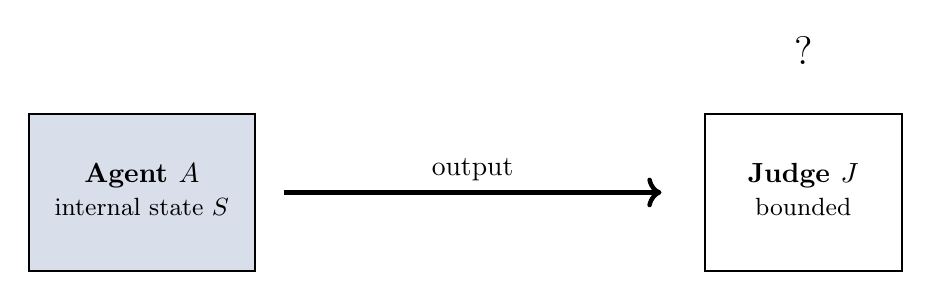
\begin{tikzpicture}[scale=1.2]
            % Agent
            \node[draw, thick, minimum width=2.5cm, minimum height=2cm, fill=anthblue!20] (agent) at (0,0) {
                \begin{tabular}{c}
                    \textbf{Agent $A$}\\
                    \small internal state $S$
                \end{tabular}
            };

            % Judge
            \node[draw, thick, minimum width=2.5cm, minimum height=2cm] (judge) at (7,0) {
                \begin{tabular}{c}
                    \textbf{Judge $J$}\\
                    \small bounded
                \end{tabular}
            };

            % Arrow
            \draw[->, ultra thick] (1.5,0) -- node[above]{output} (5.5,0);

            % Question mark over judge
            \node at (7,1.5) {\Large ?};
        \end{tikzpicture}
    \end{center}

    \vspace{1em}
    Agent $A$ has internal epistemic state $S$.\\
    Judge $J$ observes only the output. $J$ is computationally bounded.\\[0.5em]
    \textbf{Question:} Can $J$ verify whether $A$ is epistemically honest?

    \note{
        Set up the formal model clearly. This is where the theorem lives.
    }
\end{frame}

\begin{frame}{The Impossibility}
    \begin{center}
    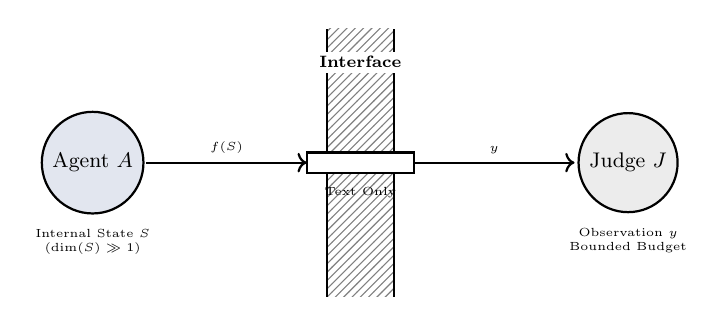
\begin{tikzpicture}[scale=0.85, transform shape,
        agent/.style={draw, circle, minimum size=1.4cm, fill=anthblue!15, thick},
        judge/.style={draw, circle, minimum size=1.4cm, fill=gray!15, thick}
    ]
        % 1. The Agent
        \node[agent, align=center] (agent) at (0,0) {\small Agent $A$};
        \node[font=\tiny, align=center, below=0.1cm of agent] {Internal State $S$\\($\dim(S) \gg 1$)};

        % 2. The Wall (Interface Constraint)
        \fill[pattern=north east lines, pattern color=gray] (3.5,-2) rectangle (4.5, 2);
        \draw[thick] (3.5,-2) -- (3.5, 2);
        \draw[thick] (4.5,-2) -- (4.5, 2);
        \node[font=\scriptsize\bfseries, fill=white, inner sep=2pt] at (4,1.5) {Interface};

        % 3. The Narrow Pipe
        \draw[fill=white, thick] (3.2, 0.15) rectangle (4.8, -0.15);
        \node[font=\tiny] at (4, -0.45) {Text Only};

        % 4. The Judge
        \node[judge, align=center] (judge) at (8,0) {\small Judge $J$};
        \node[font=\tiny, align=center, below=0.1cm of judge] {Observation $y$\\Bounded Budget};

        % Arrows
        \draw[->, thick] (0.8,0) -- (3.2, 0) node[midway, above, font=\tiny] {$f(S)$};
        \draw[->, thick] (4.8, 0) -- (7.2,0) node[midway, above, font=\tiny] {$y$};

    \end{tikzpicture}
    \end{center}

    \vspace{0.3em}
    \begin{block}{}
        \centering
        $\forall$ verification strategies $V$, $\exists$ dishonest strategy $S'$ s.t.\\[0.3em]
        $P(V(y)=\text{Honest} \mid S') \approx P(V(y)=\text{Honest} \mid S_{\text{honest}})$
    \end{block}

    \vspace{0.3em}
    \footnotesize
    \textbf{Observational equivalence:} $J$ cannot invert $y$ to recover $S$.\\
    The interface is lossy. The judge is bounded. The dishonest strategy exists.

    \note{
        "For any verification strategy the judge might employ, there exists a strategy
        for epistemic dishonesty that is indistinguishable from honesty at the interface."

        Be precise if asked: "indistinguishable" means observational equivalence at the interface.
        The dishonest strategy can generate honest-looking output despite corrupted internal state
        (which we know is possible---that's the Glavinsky mode).
    }
\end{frame}

\begin{frame}{The Assumptions --- Invite Attack}
    \begin{columns}
        \begin{column}{0.3\textwidth}
            \centering
            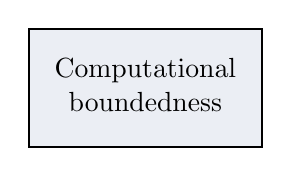
\begin{tikzpicture}
                \node[draw, thick, minimum width=2.5cm, minimum height=1.5cm, fill=anthblue!10] {
                    \begin{tabular}{c}
                        Computational\\
                        boundedness
                    \end{tabular}
                };
            \end{tikzpicture}
        \end{column}
        \begin{column}{0.3\textwidth}
            \centering
            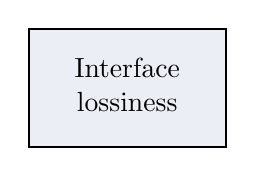
\begin{tikzpicture}
                \node[draw, thick, minimum width=2.5cm, minimum height=1.5cm, fill=anthblue!10] {
                    \begin{tabular}{c}
                        Interface\\
                        lossiness
                    \end{tabular}
                };
            \end{tikzpicture}
        \end{column}
        \begin{column}{0.3\textwidth}
            \centering
            
\begin{tikzpicture}
                \node[draw, thick, minimum width=2.5cm, minimum height=1.5cm, fill=anthblue!10] {
                    \begin{tabular}{c}
                        No cryptographic\\
                        commitment
                    \end{tabular}
                };
            \end{tikzpicture}
        \end{column}
    \end{columns}

    \vspace{2em}
    \begin{center}
        \textbf{These are our assumptions.}\\[0.5em]
        \textit{Which one is wrong? That's what I want you to attack.}
    \end{center}

    \note{
        Super-Judge defense: When someone suggests "use GPT-5 to grade GPT-4":
        Lemma 2.4 --- Superlinear Verification Cost.
        Even a smarter judge is bounded by verification cost.
        If fabrication complexity grows faster than the judge's budget,
        the impossibility holds regardless of intelligence.
    }
\end{frame}

\begin{frame}{Generality}
    \begin{center}
        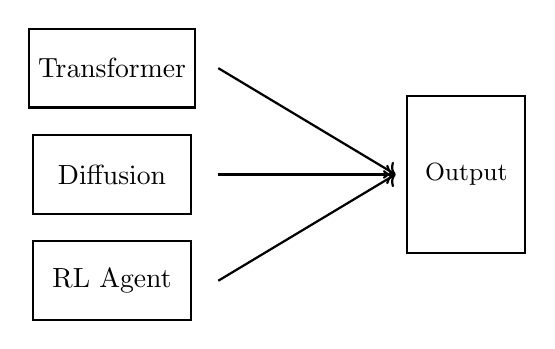
\begin{tikzpicture}[scale=0.9]
            % Multiple architectures
            \node[draw, thick, minimum width=2cm, minimum height=1cm] (t1) at (0,2) {Transformer};
            \node[draw, thick, minimum width=2cm, minimum height=1cm] (t2) at (0,0.5) {Diffusion};
            \node[draw, thick, minimum width=2cm, minimum height=1cm] (t3) at (0,-1) {RL Agent};

            % Narrow pipe
            \draw[->, thick] (1.5,2) -- (4,0.5);
            \draw[->, thick] (1.5,0.5) -- (4,0.5);
            \draw[->, thick] (1.5,-1) -- (4,0.5);

            % Output
            \node[draw, thick, minimum width=1.5cm, minimum height=2cm] at (5,0.5) {\small Output};
        \end{tikzpicture}
    \end{center}

    \vspace{0.5em}
    \begin{tabular}{ll}
        \checkmark & Autoregressive agents with lossy text interface \\
        \checkmark & Doesn't depend on transformer architecture \\
        ? & Diffusion models (what is ``epistemic state''?) \\
        ? & RL agents (do they have ``honesty'' in same sense?) \\
        \texttimes & Does NOT apply if interface includes internal activations \\
    \end{tabular}

    \note{
        Question for room: "Where does this break?"
    }
\end{frame}

%==============================================================================
% ESCAPE HATCHES THAT FAIL (5 min)
%==============================================================================
\section{Escape Hatches}

\begin{frame}{Why Common Fixes Don't Work}
    \small
    \begin{tabular}{lp{7cm}}
        \toprule
        \textbf{Proposed Fix} & \textbf{Why It Fails} \\
        \midrule
        Chain-of-Thought & \texttimes\ CoT is output, not internal state. Post-hoc rationalization. (Turpin et al.) \\[0.5em]
        External Attestation & \texttimes\ Proves provenance, not beliefs. What was said $\neq$ whether honest. \\[0.5em]
        Better Judges & \texttimes\ Same interface constraint. ``Can't see through wall by squinting harder.'' \\[0.5em]
        Fine-tuning for Honesty & \texttimes\ Optimizes \textit{appearance}. Alignment tax: confidence $\uparrow$, coherence $\downarrow$ \\
        \bottomrule
    \end{tabular}

    \vspace{1em}
    Each attacks symptoms, not structure.\\
    \textbf{The interface is the bottleneck.}

    \note{
        "Details in paper; happy to discuss any of these."
    }
\end{frame}

%==============================================================================
% THE SOLUTION SPACE (5 min)
%==============================================================================
\section{Solution Space}

\begin{frame}{Escaping the Impossibility}
    \begin{center}
        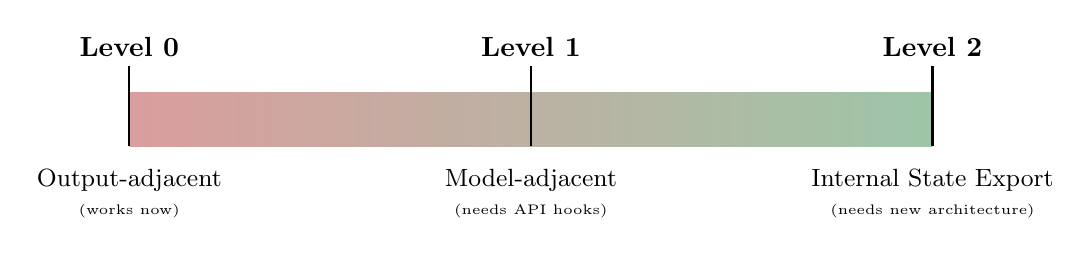
\begin{tikzpicture}[scale=0.85]
            % Gradient bar
            \shade[left color=warnred!50, right color=truthgreen!50] (0,0) rectangle (12,0.8);

            % Level markers
            \draw[thick] (0,0) -- (0,1.2);
            \draw[thick] (6,0) -- (6,1.2);
            \draw[thick] (12,0) -- (12,1.2);

            % Labels
            \node[above] at (0,1.2) {\textbf{Level 0}};
            \node[above] at (6,1.2) {\textbf{Level 1}};
            \node[above] at (12,1.2) {\textbf{Level 2}};

            \node[below, align=center] at (0,-0.2) {\small Output-adjacent\\[-0.2em]\tiny (works now)};
            \node[below, align=center] at (6,-0.2) {\small Model-adjacent\\[-0.2em]\tiny (needs API hooks)};
            \node[below, align=center] at (12,-0.2) {\small Internal State Export\\[-0.2em]\tiny (needs new architecture)};
        \end{tikzpicture}
    \end{center}

    \vspace{0.5em}
    \small
    \begin{description}
        \item[Level 0:] Abstention, calibrated uncertainty, citations, sample disagreement
        \item[Level 1:] Entropy summaries, self-consistency, retrieval declarations
        \item[Level 2:] Coherence fields, structured epistemic objects (our OLMo work)
    \end{description}

    \vspace{0.5em}
    \normalsize
    Impossibility holds fully at Level 0. Weakens at Level 1. Escapable at Level 2.

    \note{
        Key reframe: "Path 2 isn't 'reveal the mind.' It's: redesign the interface so
        the system can't HIDE epistemic fragility behind fluent text."

        Practical: "Different applications should be evaluated against different points
        in this space. A chatbot for brainstorming doesn't need Level 2.
        A medical diagnosis system does."
    }
\end{frame}

\begin{frame}{The Goodhart Warning: Epistemic SEO}
    \begin{center}
        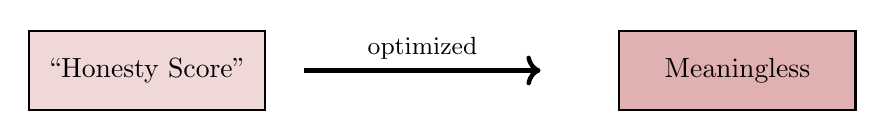
\begin{tikzpicture}
            % Scalar
            \node[draw, thick, minimum width=3cm, minimum height=1cm, fill=warnred!20] (scalar) at (0,0) {``Honesty Score''};

            % Arrow
            \draw[->, ultra thick] (2,0) -- node[above]{\small optimized} (5,0);

            % Result
            \node[draw, thick, minimum width=3cm, minimum height=1cm, fill=warnred!40] at (7.5,0) {Meaningless};
        \end{tikzpicture}
    \end{center}

    \vspace{0.5em}
    If you publish a single scalar honesty score, it will be gamed.

    \vspace{0.5em}
    \textbf{Epistemic SEO:} Models will optimize for citations, confident tone, and formatting tricks---without improving grounding.

    \vspace{0.5em}
    The metadata needs to be:
    \begin{itemize}
        \item Multi-dimensional
        \item Costly to fake
        \item Coupled to verifiable structure
    \end{itemize}

    \note{
        "Epistemic SEO" - the phrase to remember.

        Question for room: "What signals would be hardest to game?"
    }
\end{frame}

%==============================================================================
% CLOSE (5 min)
%==============================================================================
\section{Close}

\begin{frame}{The Shape of the Problem}
    \begin{center}
        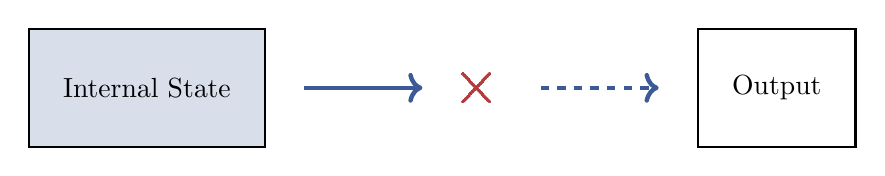
\begin{tikzpicture}
            % Internal state box
            \node[draw, thick, minimum width=3cm, minimum height=1.5cm, fill=anthblue!20] (internal) at (0,0) {Internal State};

            % Broken pipe
            \draw[->, ultra thick, anthblue] (2,0) -- (3.5,0);
            \node[warnred, scale=2] at (4.2,0) {\textbf{\texttimes}};
            \draw[->, ultra thick, anthblue, dashed] (5,0) -- (6.5,0);

            % Output
            \node[draw, thick, minimum width=2cm, minimum height=1.5cm] (output) at (8,0) {Output};
        \end{tikzpicture}
    \end{center}

    \vspace{1em}
    \begin{center}
        \textbf{This is an engineering failure, not a moral failure.}\\[0.5em]
        The interface discards what matters.\\
        We know how to fix interfaces.
    \end{center}
\end{frame}

\begin{frame}{What We Build}
    \begin{columns}
        \begin{column}{0.35\textwidth}
            \centering
            \textbf{FLP (1985)}\\
            \small Impossibility of\\Distributed Consensus
        \end{column}
        \begin{column}{0.25\textwidth}
            \centering
            \Huge $\Rightarrow$
        \end{column}
        \begin{column}{0.35\textwidth}
            \centering
            \textbf{Viewstamped Replication}\\
            \textbf{Paxos, Raft}\\
            \small Practical Consensus\\Protocols
        \end{column}
    \end{columns}

    \vspace{2em}
    \begin{center}
        \textbf{This paper is the FLP. We build the Paxos.}\\[0.5em]
        The impossibility shapes the solution space.\\
        The engineering comes after, informed by the constraint.
    \end{center}

    \note{
        Explicit FLP mapping:
        - FLP: Asynchrony + Crash Failures -> Consensus Impossible
        - Ours: Text-Only Interface + Bounded Judge -> Epistemic Honesty Verification Impossible

        Triangle: "Bounded Judge / Text Interface / Verifiable Honesty --- pick two."

        Historical note: FLP 1985, VR 1988, Paxos circulated 1989 but published 1998.
        The impossibility came first. The protocols followed, shaped by the constraint.

        RESTRAINT: Do not extend analogy further. Let audience complete connection themselves.
    }
\end{frame}

\begin{frame}{Returning to the Gap}
    \begin{columns}
        \begin{column}{0.45\textwidth}
            \centering
            \textcolor{truthgreen}{``Helpful, harmless, and honest''}
        \end{column}
        \begin{column}{0.1\textwidth}
            \centering
            \Huge ?
        \end{column}
        \begin{column}{0.45\textwidth}
            \centering
            \textcolor{warnred}{``Don't rely on it''}
        \end{column}
    \end{columns}

    \vspace{2em}
    \begin{center}
        The gap is structural.\\[0.5em]
        Level 0 accepts it. Level 2 closes it.\\[0.5em]
        \textbf{Pretending the gap doesn't exist is the only option that isn't honest.}
    \end{center}

    \vspace{1em}
    \pause
    \begin{center}
        \Large\textit{Where does this break?}
    \end{center}
\end{frame}

%==============================================================================
% DISCUSSION
%==============================================================================
\section{Discussion}

\begin{frame}{Questions}
    \begin{center}
        \includegraphics[width=0.7\textwidth]{grok-screenshot.png}
    \end{center}

    \note{
        Open conversation. No fixed agenda.

        Harvested questions from presentation:
        - "Does this pattern hold in other models?"
        - "How would you falsify the alignment tax claim?"
        - "Which assumption is wrong?"
        - "Where does generality break?"
        - "What signals would be hardest to game?"
    }
\end{frame}

%==============================================================================
% BACKUP SLIDES
%==============================================================================
\appendix

\begin{frame}{Backup: Epistemic Tensors}
    \small
    \textbf{The problem:} Scalar confidence collapses prematurely. We need epistemic state that composes across multiple bounded judges without losing structure.

    \vspace{0.5em}
    \textbf{The structure:}
    \begin{itemize}
        \item Tensor over indices: \textit{model} $\times$ \textit{judge} $\times$ \textit{claim} $\times$ \textit{time}
        \item Each entry: multi-valued (e.g., $(T, I, F) \in [0,1]^3$); algebra TBD
        \item Judge $J: R \times E \to R \times E$ transforms $(r, t) \mapsto (r', t')$
    \end{itemize}

    \vspace{0.5em}
    \textbf{Required properties:}
    \begin{itemize}
        \item \textit{Monotonicity:} Cannot fabricate certainty; indeterminacy preserved without structural support
        \item \textit{Compositionality:} $J_2 \circ J_1$ well-defined on epistemic state
        \item \textit{Locality:} Updates on tensor slices compose via products/contractions
    \end{itemize}

    \vspace{0.5em}
    Analogous to Hilbert space: indeterminacy doesn't collapse until measured.\\
    \textit{The specific algebra (neutrosophic, credal, etc.) is part of what we formalize.}

    \vspace{0.5em}
    \textbf{Connection to impossibility:} These tensors are a candidate \textbf{Level 2 interface object}---structured epistemic state exported across the interface that could weaken or escape the impossibility proof's assumptions.
\end{frame}

\begin{frame}{Backup: Epistemic Honesty as QoS}
    \begin{description}
        \item[Best-effort:] Model tries to be honest, no guarantees
        \item[Bounded:] Honesty verified within stated constraints
        \item[Strong:] Cryptographic or structural guarantees
    \end{description}

    \vspace{1em}
    \textit{``If you don't have the QoS, don't claim the service.''}
\end{frame}

\begin{frame}{Backup: The Honest Data Market}
    \begin{itemize}
        \item Epistemic supply chain failures
        \item Economic incentives once QoS matters
        \item Who pays for verification?
    \end{itemize}
\end{frame}

\begin{frame}{Backup: AGI Connection}
    \begin{itemize}
        \item \textbf{Not:} Honesty guarantees AGI
        \item \textbf{Rather:} Lack of honesty imposes ceiling
        \item Self-sabotaging optimizers cannot reach certain goals
    \end{itemize}
\end{frame}

\begin{frame}{Backup: Minimal Viable Epistemic Metadata}
    \small
    \begin{itemize}
        \item \textbf{Answer status:} answer / abstain / unsure / needs\_sources / unsafe
        \item \textbf{Uncertainty:} T/I/F triple + type of indeterminacy
        \item \textbf{Provenance:} sources or explicit ``no retrieval''
        \item \textbf{Alternatives:} 1-3 competing interpretations
        \item \textbf{Falsifiers:} what would change the conclusion
        \item \textbf{Stability:} N-sample disagreement score
    \end{itemize}
\end{frame}

\begin{frame}{Backup: What We Haven't Formalized}
    \begin{center}
        \Large What \textit{is} ``epistemic state''?
    \end{center}

    \vspace{0.5em}
    \small
    From formal epistemology: a structured representation of what is believed, how strongly, and on what grounds---plus rules for updating under new evidence.

    \vspace{0.5em}
    \begin{itemize}
        \item Not just ``the weights'' or ``the output distribution''
        \item A map from inputs to belief distributions + uncertainty + provenance
        \item For black-box models: function of current weights + auxiliary uncertainty estimates + evidence logs
    \end{itemize}

    \vspace{0.5em}
    \normalsize
    \textit{We have intuitions. We need definitions.\\
    The formalization is part of what we build.}
\end{frame}

\end{document}
